
\documentclass[11pt]{article}

\usepackage[a4paper]{geometry}	%page margins
\usepackage{graphicx}
\usepackage{fancyhdr}
\usepackage{color}
\usepackage{lastpage}
\usepackage{titling}
\usepackage{amssymb}
\usepackage{amsmath}
\usepackage[utf8]{inputenc}
%\usepackage[utf8x]{inputenc}
\usepackage[T1]{fontenc}
\usepackage{graphicx}
\usepackage{cmap}

\usepackage{gensymb}

\usepackage{color}
\usepackage{hyperref}

\usepackage{listings}



%\DeclareUnicodeCharacter{00A0}{ }

\title{Relazione RO per l'A.A. 2016/2017}
\author{Leonardo Brutesco}

\graphicspath{ {images/} }

\hypersetup{
	colorlinks=true,
	linktoc=true,
	linkcolor=blue,
	linktocpage=true
}
	%hidelinks=true
	%citecolor=black
	%filecolor=black
	%urlcolor=black
\lstset{
	basicstyle={Ubuntu mono}
	columns=fullflexible,
	frame=single,
	breaklines=true,
	postbreak=\mbox{\textcolor{red}{$\hookrightarrow$}\space},
}
	%basicstyle=\ttfamily,


\newcommand{\RealSet}{\mathbb{R}}
\newcommand{\BinSet}{\{0,1\}}
\newcommand{\NaturalSet}{\mathbb{N}}
\newcommand{\IntegerSet}{\mathbb{Z}}
 


\newcommand{\matNum}{1097942}
\newcommand{\matricola}{Mat: \matNum}



\renewcommand{\headrulewidth}{0.4pt}
\renewcommand{\footrulewidth}{0.4pt}


\pagestyle{fancy}
\fancyhead{}
\fancyfoot{}
%\fancyfoot[R]{\thepage}


\fancyhead[L]{\thetitle}
\fancyhead[R]{\theauthor\ [\matricola]}
\fancyfoot[R]{Pagina \thepage\ di \pageref{LastPage}}

\begin{document}


%%%%%%%%%%%%%%%%%%%%
% TITLE
%%%%%%%%%%%%%%%%%%%%

%	\maketitle
\begin{center}
	\hspace{0pt}
	\vfill
	\Huge{
		\textbf{\thetitle} \\
		\LARGE{\textbf{Progetto: texture atlas}} \\
		\ \newline \newline \newline
		\Large{	Studente: \textbf{\theauthor} } \\
		\normalsize{{Matricola: \textbf{\matNum}} }
	}
	\vfill
	\hspace{0pt}
	%\vspace*{\fill}
	%\pagebreak
\end{center}
\newpage


%%%%%%%%%%%%%%%%%%%%
% TOC
%%%%%%%%%%%%%%%%%%%%


\tableofcontents    
\newpage



%%%%%%%%%%%%%%%%%%%%
% DESCRIZIONE
%%%%%%%%%%%%%%%%%%%%

% descrizione + caratteristiche (?)

\section{Descrizione del problema}



Il problema trattato è quello delle texture atlas, ovvero immagini di dimensioni spesso notevoli utilizzate come raccoglitori di altre immagini, utili per accelerare l’accesso (soprattutto da parte della GPU) alle texture utilizzate da parte dei programmi. \\
Si vuole trovare la minima lunghezza D tale che un’immagine quadrata di dimensioni DxD contenga tutte le texture comprese in un insieme dato. \\
Il vincolo principale del problema è che D deve poter contenere tutte le immagini, quindi D dev’essere almeno uguale alla posizione+dimensione (in ascissa e ordinata) di ogni immagine. \\
Il secondo vincolo principale comporta invece la non sovrapposizione di due texture. Questo vincolo è presente per ogni coppia di immagini diverse dell’insieme. \\
\ \\
Altri vincoli secondari riguardano tre opzioni del modello, ovvero la possibilità di permettere rotazioni delle texture, il tener conto di un piccolo bordo per ogni immagine e limitare i valori assegnabili a D alle sole potenze di 2.


\newpage








  % descrizione + caratteristiche (?)

	\section{Descrizione del problema}


 
Il problema in esame richiede di trovare la minima lunghezza D per cui un'immagine D*D contenga tutte le immagini facenti parte della texture atlas. \\
vincolo principale del problema è che D deve poter contenere tutte le immagini, quindi D dev'essere almeno uguale alla posizione+dimensione (W, H) di ogni immagine. \\
altro vincolo comporta la non sovraposizione per ogni coppia di immagini dell'insieme. \\



	\newpage



  %descrizione modello + spiegazione (vincoli etc)

	\section{Modello (matematico)}


\begin{align*}	% l'asterisco toglie il numero alle righe (: equazioni)
minimize \ \ D \\	% & per allineare
%
0 \leq X_i           \ \ \ \ \   &\forall{ i \in I} \\
X_i +W_i \leq D      \ \ \ \ \   &\forall{ i \in I} \\
0 \leq Y_i           \ \ \ \ \   &\forall{ i \in I} \\
Y_i +H_i \leq D      \ \ \ \ \   &\forall{ i \in I} \\ \\
%
%
Cx_{i,j} = X_i - (X_j + W_j)       \ \ \ \ \   &\forall{ i \in I, j \in J: i \neq j} \\
Cy_{i,j} = Y_i - (Y_j + H_j)       \ \ \ \ \   &\forall{ i \in I, j \in J: i \neq j} \\ \\
%
%
Cx_{i,j} \leq M *befX_{i,j} -1           \ \ \ \ \   &\forall{ i \in I, j \in J: i \neq j} \\
Cx_{i,j} \geq 0 + M*(1-befX_{i,j})       \ \ \ \ \   &\forall{ i \in I, j \in J: i \neq j} \\ \\
%
%
Cy_{i,j} \leq M *befY_{i,j} -1           \ \ \ \ \   &\forall{ i \in I, j \in J: i \neq j} \\
Cy_{i,j} \geq 0 + M*(1-befY_{i,j})       \ \ \ \ \   &\forall{ i \in I, j \in J: i \neq j} \\ \\
%
%
(1-befX_{i,j})+(1-befX_{j,i})+ \ \ \ \ & \\ (1-befY_{i,j})+(1-befY_{j,i}) \leq 3       \ \ \ \ \   &\forall{ i \in I, j \in J: i \neq j} \\ \\
%
%s.t. l1{i in I, j in I:i!=j}: (Cx[i,j]) <= bigM*befX[i,j]+-1                 ;			#problema con una unità?
%s.t. l2{i in I, j in I:i!=j}: (Cx[i,j]) >= 0             -bigM*(1-befX[i,j]);		#problema con una unità?
%
%
\\
X_i \in \NaturalSet      \ \ \ \ &\forall{i \in I} \\
Y_i \in \NaturalSet      \ \ \ \ &\forall{i \in I} \\
Cx_{i,j} \in \IntegerSet \ \ \ \ &\forall{i \in I,j \in I} \\
Cy_{i,j} \in \IntegerSet \ \ \ \ &\forall{i \in I,j \in I} \\
BefX{i,j} \in \BinSet    \ \ \ \ &\forall{i \in I,j \in I} \\
BefY{i,j} \in \BinSet    \ \ \ \ &\forall{i \in I,j \in I} 
%
 \end{align*}



		\subsection{Variabili Decisionali}

		Bef{x,y}
		\subsection{Parametri}
		W
		H
		useBleding
		usePowTwo
		useRotation
		\subsection{Vincoli e funzione obiettivo}
		min D

		Cx Cy
		\newpage


%  (procedimenti per arrivare al risultato?) come (è/ho(?))) fatto


	\section{Implementazione in AMPL}
		\subsection{File .mod}
		%input diretto dei file?
		
		\subsection{File .dat}

		\subsection{File .run}
		\newpage


\section{Dati d'esempio}

	Esistono 6 file di dati d'esempio che prendono le immagini da 3 set distinti; a coppie, i file richiedono la soluzione su uno stesso set di immagini, ma con parametri diversi. \\
	Per ogni set vengono presentati i dati distinti con i parametri utilizzati nei relativi file. Quindi si mostrerà l'output del programma \texttt{amplide} seguito dai valori delle variabili della soluzione. \\
	La soluzione si compone del valore della funzione obiettivo, che coincide con la variabile D, seguito da una tupla nel formato <nome, X, Y, larghezza, altezza, rotazione> per ogni immagine. \\
	Seguirà poi un confronto grafico tra le soluzioni dei vari problemi con parametri diversi.


%%%%%%%%%%
%% SET 1
%%%%%%%%%%

	\subsection{Set 1}
	%\subsubsection{Immagini}
\iffalse
	Nel set sono presenti 6 immagini:
	\begin{itemize}
		\itemsep0em
		\item \texttt{a:\ 16x16};
		\item \texttt{b:\ \ 8x16};
		\item \texttt{c:\ \ 8x\ 8};
		\item \texttt{d:\ \ 5x25};
		\item \texttt{e:\ 72x32};
		\item \texttt{f:\ 32x32};
	\end{itemize}
\fi
%
Dati del set di immagini:  \\
%

\begin{table}[h!]
\centering
\footnotesize
\begin{tabular}{l|r|r}
\multicolumn{3}{c}{\textbf{Immagini}} \\ 
%\hline
id & larghezza & altezza \\
\hline
a & 16 & 16 \\
		 b & 8&16\\
		 c & 8& 8\\
		 d & 5&25\\
		 e & 72&32\\
		 f & 32 &32\\
\end{tabular}
\end{table}
%
%\subsubsection{Risultati}


\noindent Parametri, Output e Soluzione dei 2 problemi: 

\begin{table}[h]
\centering
\footnotesize
\begin{tabular}{p{5cm}|p{5cm}}
%\hline
\textbf{Problema 1} & \textbf{Problema 2} \\
\hline
\multicolumn{2}{|c|}{Parametri} \\ 
\hline
allowRotations = 0,\newline
useNoBleeding = 0,\newline
usePowersOf2 = 1;	& 
allowRotations = 1,\newline
useNoBleeding = 1,\newline
usePowersOf2 = 1;	\\
\hline
\multicolumn{2}{|c|}{Output AMPL} \\
\hline
\texttt{69 MIP simplex iterations \newline
0 branch-and-bound nodes \newline
D = 128}
&
\texttt{69 MIP simplex iterations \newline
0 branch-and-bound nodes \newline
D = 128}
\\
\hline
\multicolumn{2}{|c|}{Soluzione} \\
\hline
\texttt{128 \newline
109,1,16,16,0\newline
37,0,8,16,0\newline
0,0,8,8,0\newline
32,0,5,25,0\newline
37,16,72,22,0\newline
0,8,32,32,0}
&
\texttt{128 \newline
109,1,16,16,0\newline
37,0,8,16,0\newline
0,0,8,8,0\newline
32,0,5,25,0\newline
37,16,72,22,0\newline
0,8,32,32,0}
\\
   \hline
\end{tabular}
\end{table}

	%\subsubsection{Risultati}



















%%%%%%%%%%
%% SET 2
%%%%%%%%%%

	\subsection{Set 1}
	%\subsubsection{Immagini}
\iffalse
	Nel set sono presenti 6 immagini:
	\begin{itemize}
		\itemsep0em
		\item \texttt{a:\ 16x16};
		\item \texttt{b:\ \ 8x16};
		\item \texttt{c:\ \ 8x\ 8};
		\item \texttt{d:\ \ 5x25};
		\item \texttt{e:\ 72x32};
		\item \texttt{f:\ 32x32};
	\end{itemize}
\fi
%
Dati del set di immagini:  \\
%

\begin{table}[h!]
\centering
\footnotesize
\begin{tabular}{l|r|r}
\multicolumn{3}{c}{\textbf{Immagini}} \\ 
%\hline
id & larghezza & altezza \\
\hline
a & 16 & 16 \\
		 b & 8&16\\
		 c & 8& 8\\
		 d & 5&25\\
		 e & 72&32\\
		 f & 32 &32\\
\end{tabular}
\end{table}
%
%\subsubsection{Risultati}


\noindent Parametri, Output e Soluzione dei 2 problemi: 

\begin{table}[h]
\centering
\footnotesize
\begin{tabular}{p{5cm}|p{5cm}}
%\hline
\textbf{Problema 1} & \textbf{Problema 2} \\
\hline
\multicolumn{2}{|c|}{Parametri} \\ 
\hline
allowRotations = 0,\newline
useNoBleeding = 0,\newline
usePowersOf2 = 1;	& 
allowRotations = 1,\newline
useNoBleeding = 1,\newline
usePowersOf2 = 1;	\\
\hline
\multicolumn{2}{|c|}{Output AMPL} \\
\hline
\texttt{69 MIP simplex iterations \newline
0 branch-and-bound nodes \newline
D = 128}
&
\texttt{69 MIP simplex iterations \newline
0 branch-and-bound nodes \newline
D = 128}
\\
\hline
\multicolumn{2}{|c|}{Soluzione} \\
\hline
\texttt{128 \newline
109,1,16,16,0\newline
37,0,8,16,0\newline
0,0,8,8,0\newline
32,0,5,25,0\newline
37,16,72,22,0\newline
0,8,32,32,0}
&
\texttt{128 \newline
109,1,16,16,0\newline
37,0,8,16,0\newline
0,0,8,8,0\newline
32,0,5,25,0\newline
37,16,72,22,0\newline
0,8,32,32,0}
\\
   \hline
\end{tabular}
\end{table}

	%\subsubsection{Risultati}






%%%%%%%%%%
%% SET 3
%%%%%%%%%%

	\subsection{Set 1}
	%\subsubsection{Immagini}
\iffalse
	Nel set sono presenti 6 immagini:
	\begin{itemize}
		\itemsep0em
		\item \texttt{a:\ 16x16};
		\item \texttt{b:\ \ 8x16};
		\item \texttt{c:\ \ 8x\ 8};
		\item \texttt{d:\ \ 5x25};
		\item \texttt{e:\ 72x32};
		\item \texttt{f:\ 32x32};
	\end{itemize}
\fi
%
Dati del set di immagini:  \\
%

\begin{table}[h!]
\centering
\footnotesize
\begin{tabular}{l|r|r}
\multicolumn{3}{c}{\textbf{Immagini}} \\ 
%\hline
id & larghezza & altezza \\
\hline
a & 16 & 16 \\
		 b & 8&16\\
		 c & 8& 8\\
		 d & 5&25\\
		 e & 72&32\\
		 f & 32 &32\\
\end{tabular}
\end{table}
%
%\subsubsection{Risultati}


\noindent Parametri, Output e Soluzione dei 2 problemi: 

\begin{table}[h]
\centering
\footnotesize
\begin{tabular}{p{5cm}|p{5cm}}
%\hline
\textbf{Problema 1} & \textbf{Problema 2} \\
\hline
\multicolumn{2}{|c|}{Parametri} \\ 
\hline
allowRotations = 0,\newline
useNoBleeding = 0,\newline
usePowersOf2 = 1;	& 
allowRotations = 1,\newline
useNoBleeding = 1,\newline
usePowersOf2 = 1;	\\
\hline
\multicolumn{2}{|c|}{Output AMPL} \\
\hline
\texttt{69 MIP simplex iterations \newline
0 branch-and-bound nodes \newline
D = 128}
&
\texttt{69 MIP simplex iterations \newline
0 branch-and-bound nodes \newline
D = 128}
\\
\hline
\multicolumn{2}{|c|}{Soluzione} \\
\hline
\texttt{128 \newline
109,1,16,16,0\newline
37,0,8,16,0\newline
0,0,8,8,0\newline
32,0,5,25,0\newline
37,16,72,22,0\newline
0,8,32,32,0}
&
\texttt{128 \newline
109,1,16,16,0\newline
37,0,8,16,0\newline
0,0,8,8,0\newline
32,0,5,25,0\newline
37,16,72,22,0\newline
0,8,32,32,0}
\\
   \hline
\end{tabular}
\end{table}

	%\subsubsection{Risultati}



\newpage

\subsection{Confronti grafici}

%\begin{figure}[h!]
% \noindent Confronto grafico: \\
Di seguito le immagini ottenute dalle soluzioni dei due problemi. \\
In sequenza, da sinistra a destra, dall'alto al basso, le immagini rispettivamente del Problema 1, 2, 3, 4, 5, 6. \\
 In ogni immagine, per ogni texture del texture atlas viene utilizzato un colore diverso; il contorno bianco indica l'eventuale bordo necessario per evitare l'effetto bleeding. 
	 %A sinistra il 1\degree{} problema, a destra il 2\degree. \\
\subsubsection{Problemi 1 e 2}
\vcenter{
\centering
	
\includegraphics[width=5cm]{results01}
	\hspace{1cm}
	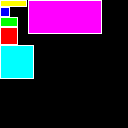
\includegraphics[width=5cm]{results02}
}\\
\subsubsection{Problemi 3 e 4}
\vcenter{
\centering
	
\includegraphics[width=5cm]{results01}
	\hspace{1cm}
	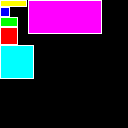
\includegraphics[width=5cm]{results02}
} \\
\subsubsection{Problemi 5 e 6}
\vcenter{
\centering
	
\includegraphics[width=5cm]{results01}
	\hspace{1cm}
	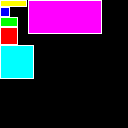
\includegraphics[width=5cm]{results02}
}




\iffalse
\newpage
{\centering
	
\includegraphics[width=4cm]{results01}
	\hspace{1cm}
	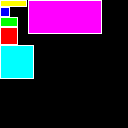
\includegraphics[width=4cm]{results02}
	\caption{\\Le immagini ottenute dalle soluzioni dei due problemi. 
	 A sinistra il 1\degree{} problema, a destra il 2\degree. \\
	 { %\footnotesize
	 Per ogni immagine viene utilizzato un colore diverso; il contorno bianco indica il bordo necessario per evitare l'effetto bleeding.
	 } } }
%\end{figure}
\begin{figure}[h!]
% \noindent Confronto grafico: \\
{\centering
	
\includegraphics[width=4cm]{results01}
	\hspace{1cm}
	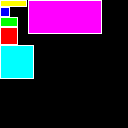
\includegraphics[width=4cm]{results02}
	\caption{\\Le immagini ottenute dalle soluzioni dei due problemi. 
	 A sinistra il 1\degree{} problema, a destra il 2\degree. \\
	 { %\footnotesize
	 Per ogni immagine viene utilizzato un colore diverso; il contorno bianco indica il bordo necessario per evitare l'effetto bleeding.
	 } } }
\end{figure}


\begin{figure}[h!]
% \noindent Confronto grafico: \\
{\centering
	
\includegraphics[width=4cm]{results01}
	\hspace{1cm}
	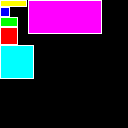
\includegraphics[width=4cm]{results02}
	\caption{\\Le immagini ottenute dalle soluzioni dei due problemi. 
	 A sinistra il 1\degree{} problema, a destra il 2\degree. \\
	 { %\footnotesize
	 Per ogni immagine viene utilizzato un colore diverso; il contorno bianco indica il bordo necessario per evitare l'effetto bleeding.
	 } } }
\end{figure}


\fi






\iffalse

ampl: include atlas.run;
CPLEX 12.6.3.0: optimal integer solution; objective 128
69 MIP simplex iterations
0 branch-and-bound nodes
No basis.
D = 128

ampl: include atlas.run;
CPLEX 12.6.3.0: optimal integer solution; objective 128
110 MIP simplex iterations
0 branch-and-bound nodes
No basis.
D = 128

ampl: include atlas.run;
CPLEX 12.6.3.0: optimal integer solution; objective 228
16295 MIP simplex iterations
2405 branch-and-bound nodes
No basis.
D = 228

ampl: include atlas.run;
CPLEX 12.6.3.0: optimal integer solution; objective 224
1084 MIP simplex iterations
277 branch-and-bound nodes
No basis.
D = 224

ampl: include atlas.run;
CPLEX 12.6.3.0: optimal integer solution; objective 198
4403 MIP simplex iterations
1423 branch-and-bound nodes
No basis.
D = 198

ampl: include atlas.run;
CPLEX 12.6.3.0: optimal integer solution; objective 256
222 MIP simplex iterations
0 branch-and-bound nodes
No basis.
D = 256
























128,0
109,1,16,16,0
37,0,8,16,0
0,0,8,8,0
32,0,5,25,0
37,16,72,22,0
0,8,32,32,0

128,1
0,27,18,18,0
0,17,18,10,1
0,7,10,10,0
0,0,27,7,1
28,4,74,24,0
0,45,34,34,0

228,1
98,0,130,34,0
194,100,34,34,0
132,34,66,66,0
132,100,34,98,1
194,134,34,66,0
98,58,34,170,1
0,98,98,130,0
0,0,98,98,0

224,0
32,0,128,32,0
192,0,32,32,0
96,64,64,64,0
0,192,96,32,0
0,0,32,64,0
56,32,168,32,0
0,64,96,128,0
97,128,96,96,0

198,1
180,0,18,34,0
164,164,34,34,0
170,0,10,10,0
169,83,7,17,0
136,0,34,66,0
0,0,34,170,1
34,100,130,98,1
34,0,98,98,0

256,1
98,0,18,34,0
10,0,34,34,0
0,0,10,10,0
0,17,7,17,0
0,170,34,66,0
116,0,34,170,1
158,0,98,130,0
0,34,98,98,0


\fi











	\newpage




	\section{Osservazioni}
	
Mettendo a confronto i dati delle soluzioni dei problemi, si possono comparare in maniera critica i risultati e l'esecuzione del modello e ottenere delle osservazioni (alcune ovvie ma comunque degne di nota).\\
Dai 6 problemi si può notare che:
\begin{enumerate}
	\item limitare i valori assegnabili a D riduce di molto la complessità del modello, poiché si devono controllare pochi valori e ciò fa sì che si riduca il numero di MIP simplex iterations e di nodi branch-and-bound durante l'esecuzione; ciò a discapito di una soluzione sicuramente non migliore rispetto a un problema con un set di valori non limitato.
	\item richiedere un bordo per evitare l'effetto bleeding implica una soluzione probabilmente peggiore poiché, inevitabilmente, viene occupato più spazio
	\item permettere le rotazioni invece aumenta un po' la complessità del problema ma consente di trovare soluzioni migliori, poiché sono previste più possibilità per i valori delle soluzioni.
\end{enumerate}
%osservazioni sulla velocità usando solo potenze di 2
\ \\
%e permettendo le rotazioni aumenta la complessità


	%\newpage



\section{Funzionalità Aggiuntive}

\subsection{makeImg}
È stato sviluppato un piccolo programma JavaScript di supporto per la creazione di un'immagine dalle informazioni della soluzione. L'immagine così creata permette una migliore comprensione della soluzione di ogni set di dati. 

\subsection{soluz\_\#\#.txt}
Lo script .run crea un file di nome soluz\_\#\#.txt contenente i dati della soluzioni per disporre in maniera ottimale le texture. \\
Il contenuto di questo file può essere inserito in makeImg per creare una immagine relativa alla soluzione.

\newpage


\iffalse
  % risultati
	\section{Risultati del problema}
	\newpage

	  %commenti
	\section{Osservazioni}
	\newpage
\fi
	
	\appendix
%	\section{appendice?}

% \listoffigures

	\newpage
\end{document}
